\documentclass[11pt, oneside]{article}
\usepackage[letterpaper, margin=2cm]{geometry}
\usepackage{MATH566}
%\usepackage{sagetex}

\begin{document}
\noindent \textbf{\Large{Caleb Logemann \\
MATH 566 Discrete Optimization\\
Homework 9
}}

%\lstinputlisting[language=Sage]{03_2.sage}
\begin{enumerate}
  \item % #1 Done
    Implement Directed Minimum Mean Cycle in Sage. 
    Before implementing the algorithm, show that it is possible to slightly
    modify the algorithm.
    Instead of adding an extra vertex $s$ and edges from $s$ to all other
    vertices, it is possible to simply assign $F_0(v) = 0$ for all $v \in V$ at
    the beginning.
    This avoids the hassle with adding an extra vertex.
    But it requires an argument that the algorithm is still correct.

    In the initial algorithm in the notes we consider a vertex $s$ from which
    all other vertices can be can be reached.
    If instead we consider potentially starting at any vertex, we are not
    required to introduce a new vertex.
    This also implies that $F_0(v) = 0$ for all vertices because there always
    exists a walk of length zero from a vertex to itself, the empty walk.
    In this new setup $F_k(v)$ now represents the minimum cost walk of length
    $k$ from any vertex to $v$.
    The rest of the algorithm works as intended, the vertex that realizes
    \[
      \min*[v \in V]{\max*[k, F_k(v) \neq \infty]{\frac{F_n(v) - F_k(v)}{n - k}}}
    \]
    will be on the minimum mean cost cycle.

    The following function performs the minimum mean cost cycle algorithm
    as described in the notes with the modification described above.
    \lstinputlisting[language=Sage]{Sage/minimumMeanCostCycle.sage}
    This script runs this algorithm on 3 test graphs.
    \lstinputlisting[language=Sage]{Sage/09_1.sage}

    The output of this script is shown below.
    \begin{verbatim}
      Launched png viewer for Graphics object consisting of 15 graphics primitives
      Mu= 3/4
      Launched png viewer for Graphics object consisting of 13 graphics primitives
      Launched png viewer for Graphics object consisting of 29 graphics primitives
      Mu= 1
      Launched png viewer for Graphics object consisting of 19 graphics primitives
      Launched png viewer for Graphics object consisting of 16 graphics primitives
      This graph is acyclic
    \end{verbatim}
    The scipt also produces the following images.
    \begin{center}
      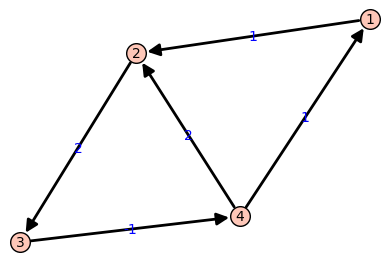
\includegraphics[scale=.5]{Figures/09_1.png}
      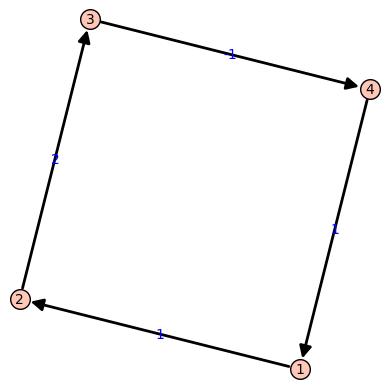
\includegraphics[scale=.5]{Figures/09_2.png} \\
      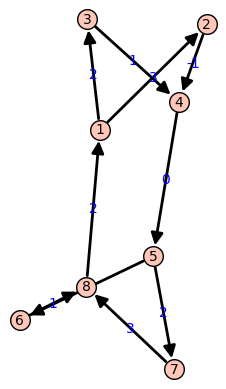
\includegraphics[scale=.5]{Figures/09_3.png}
      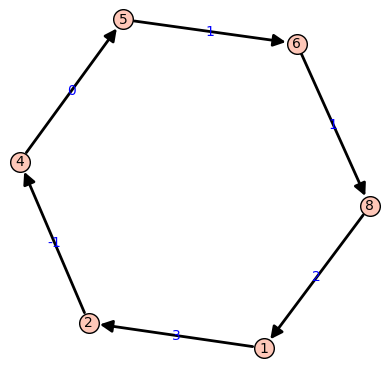
\includegraphics[scale=.5]{Figures/09_4.png} \\
      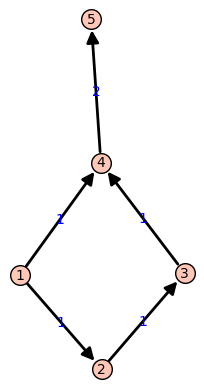
\includegraphics[scale=.5]{Figures/09_5.png}
    \end{center}

  \item % #2 Done
    Show that in integer program, it is possible to express the following constraint:
    \[
      x \in [100,200]  \cup [300,400]
    \]
    in other words
    \[
      100 \leq x \leq 200   \text{ or } 300 \leq x \leq 400
    \]
    How to express the constraint \emph{without} using \emph{or}?\\
    % Hint: use additional integer variable z \in \{0,1\}, consider z and (1-z).

    First of all it can be see that $x \ge 100$ and $x \le 400$ unconditionally
    as both intervals satisfy these conditions.
    Assuming these inequalities the system can be simplified to
    either $x \le 200$ or $x \ge 300$.
    In order to express this or statement as linear constraints consider
    $z \in \ZZ$ such that $0 \le z \le 1$.
    Now the variable $z$ is a binary variable that will turn on only one
    of the previous constraints.
    Consider the system
    \begin{align*}
      x &\le 200 + Mz \\
      x &\ge 300 - M(1 - z)
    \end{align*}
    where $M$ is sufficiently large.
    In this case $M = 200$ is sufficient.
    Consider when $z = 0$, in this case these constraints become
    \begin{align*}
      x &\le 200 \\
      x &\ge 100
    \end{align*}
    This corresponds to $x \in \br{100, 200}$
    Consider the case when $z = 1$, then the constraints become
    \begin{align*}
      x &\le 400 \\
      x &\ge 300
    \end{align*}
    This corresponds to $x \in \br{300, 400}$.
    In fact when $M = 200$, these constraints don't even require the upper and
    lower bounds stated earlier.
    This constraint can be fully expressed as
    \begin{align*}
      x &\le 200 + 200z \\
      x &\ge 300 - 200(1 - z) \\
      z &\ge 0 \\
      z &\le 1 \\
      x, z &\in \ZZ
    \end{align*}
    This system is identical to the statement
    $x \in \br{100, 200} \cup \br{300, 400}$ and $x \in \ZZ$.

  \item % #3 Done
    Determine which of the matrices below are (i) unimodular, (ii) totally
    unimodular, or (iii) neither.
    Be sure to explain your answer.

    \begin{center}
      \begin{tabular}[h]{c@{\qquad}c@{\qquad}c}
        $\left(\begin{array}{rrrr}
        1 & -1 & -1 & 0\\
        -1 & 0 & 0 & 1\\
        0 & 1 & 0 & -1\\
        0 & 0 & 1 & 0\end{array}\right)$ & 
        $\left(\begin{array}{cccc}
        1 & 0 & 1 & 0\\
        0 & 1 & 0 & 0\\
        0 & 0 & 1 & 1\\
        1 & 1 & 0 & 1\end{array}\right)$ &
        $\left(\begin{array}{ccccc}
        0 & 1 & 0 & 0 & 0  \\
        1 & 0 & 1 & 0  & 0 \\
        0 & 1 & 0 & 1 & 1\\
        0 & 0 & 1 & 0 & 1\\
        0 & 0 & 1 & 1 & 0\end{array}\right) $
        \\
        \textbf{a.} &
        \textbf{b.}  &
        \textbf{c.} 
      \end{tabular}
    \end{center}

    \begin{enumerate}
      \item[(i)]
        Since these are all square matrices, they will be unimodular if their
        determinant is $\pm 1$.
        So I compute the determinants of these 3 matrices.
        First I will compute the determinant of $(a)$.
        \begin{align*}
          \det(a) &= \begin{vmatrix}
             1 & -1 & -1 &  0 \\
            -1 &  0 &  0 &  1 \\
             0 &  1 &  0 & -1 \\
             0 &  0 &  1 &  0
          \end{vmatrix}
          \intertext{Expand along first column}
          \det(a) &= 1 \times
          \begin{vmatrix}
            0 &  0 &  1 \\
            1 &  0 & -1 \\
            0 &  1 &  0
          \end{vmatrix}
          - (-1) \times
          \begin{vmatrix}
            -1 & -1 &  0 \\
             1 &  0 & -1 \\
             0 &  1 &  0
          \end{vmatrix}
          \intertext{Expand along the first column for the first determinant
            and along the last column for the second determinant}
          &=
          1 \times \p{-1 \times 
          \begin{vmatrix}
            0 &  1 \\
            1 &  0
          \end{vmatrix}}
          - (-1) \times \p{1 \times
          \begin{vmatrix}
            -1 & -1 \\
             0 &  1
          \end{vmatrix}} \\
          &= 
          1 \times \p{-1 \times -1} - (-1) \times \p{1 \times -1} \\
          &= 1 - 1 \\
          &= 0
        \end{align*}
        Since the determinant of $(a)$ is 0 this matrix is not unimodular.

        Second I will compute the determinant of $(b)$.
        \begin{align*}
          \det(b) &=
          \begin{vmatrix}
            1 & 0 & 1 & 0 \\
            0 & 1 & 0 & 0 \\
            0 & 0 & 1 & 1 \\
            1 & 1 & 0 & 1
          \end{vmatrix}
          \intertext{I will first expand along the first row.}
          \det(b) &= 1 \times
          \begin{vmatrix}
            1 & 0 & 0 \\
            0 & 1 & 1 \\
            1 & 0 & 1
          \end{vmatrix}
          + 1 \times
          \begin{vmatrix}
            0 & 1 & 0 \\
            0 & 0 & 1 \\
            1 & 1 & 1
          \end{vmatrix}
          \intertext{I will expand the first determinant along the first row
            and the second determinant along the first column}
          \det(b) &= 1 \times \p{1 \times
          \begin{vmatrix}
            1 & 1 \\
            0 & 1
          \end{vmatrix}}
          + 1 \times \p{1 \times
          \begin{vmatrix}
            1 & 0 \\
            0 & 1 \\
          \end{vmatrix}} \\
          &= 1 \times \p{1 \times 1} + 1 \times \p{1 \times 1} \\
          &= 1 + 1 \\
          &= 2
        \end{align*}
        Since the determinant of $(b)$ is 2 this matrix is not unimodular.

        Lastly I will compute the determinant of $(c)$.
        \begin{align*}
          \det(c) &=
          \begin{vmatrix}
            0 & 1 & 0 & 0 & 0 \\
            1 & 0 & 1 & 0 & 0 \\
            0 & 1 & 0 & 1 & 1 \\
            0 & 0 & 1 & 0 & 1 \\
            0 & 0 & 1 & 1 & 0
          \end{vmatrix}
          \intertext{First I will expand along the first column}
          \det(c) &= -1 \times
          \begin{vmatrix}
            1 & 0 & 0 & 0 \\
            1 & 0 & 1 & 1 \\
            0 & 1 & 0 & 1 \\
            0 & 1 & 1 & 0
          \end{vmatrix}
          \intertext{Next I will expand along the first row}
          \det(c) &= -1 \times \p{1 \times
          \begin{vmatrix}
            0 & 1 & 1 \\
            1 & 0 & 1 \\
            1 & 1 & 0
          \end{vmatrix}}
          \intertext{Expanding along the first column gives}
          \det(c) &= -1 \times \p{1 \times \p{-1 \times
          \begin{vmatrix}
            1 & 1 \\
            1 & 0
          \end{vmatrix}
          + 1 \times
          \begin{vmatrix}
            1 & 1 \\
            0 & 1 \\
          \end{vmatrix}}} \\
          &= -1 \times \p{1 \times \p{-1 \times -1 + 1 \times 1}} \\
          &= -1 \times \p{1 \times \p{1 + 1}} \\
          &= -1 \times \p{1 \times 2} \\
          &= -1 \times 2 \\
          &= -2
        \end{align*}
        Since the determinant of $(c)$ is -2 this matrix is not unimodular.

        In summary none of the matrices are unimodular.

      \item[(ii)]
        In order for a matrix to be totally unimodular every square submatrix
        must have determinant $-1$, $0$, or $1$.
        Note that since matrices $(b)$ and $(c)$ don't have a determinant
        $-1$, $0$, or $1$ when considered as a whole matrix they cannot be
        totally unimodular.
        Matrix $(a)$ which has determinant 0 can potentially be totally
        unimodular.
        In fact we see that each column has exactly one $1$ and one $-1$, so
        by a theorem in the notes $(a)$ is totally unimodular.

      \item[(iii)]
        We have shown that $(a)$ is totally unimodular but not unimodular.
        However $(b)$ and $(c)$ are neither unimodular nor totally unimodular.
    \end{enumerate}

  \item % #4 Done
    Show that $A \in \mathbb{Z}^{m \times n}$ is totally unimodular iff $[A\ I]$
    is unimodular (where $I$ is $m \times m$ unit matrix).

    \begin{proof}
      Let $A \in \ZZ^{m \times n}$ and let $I$ be the $m \times m$ identity
      matrix.
      Let $A$ be totally unimodular.
      This implies that any square submatrix has determinant $0$, $1$, or $-1$.
      Consider a $m \times m$ basis of $\br{A\ I}$.
      Clearly any basis that contains only columns of $A$ has determinant either
      $1$ or $-1$, as $A$ is totally unimodular.
      Now let this basis contain some columns of $I$.
      Let $A_b$ be the columns of $A$ in the basis and let $I_b$ be the
      columns of $I$ in the basis.
      Now this basis can be thought of as the square matrix $\br{A_b\ I_b}$.
      Let $K = \set{k : e_k \in I_b}$, which is the set of indices of vector
      in $I$ that are contained in $I_b$.
      Thus if $1 \in K$, then $e_1 = \br{1, 0, 0, \cdots}^T \in I_b$.
      Also let $K^c$ be the set of indices that are not in $K$.
      Note that $\abs{K^c}$ is equal to the number of columns of $A_b$.
      When taking the determinant of $\br{A_b\ I_b}$, it is possible to
      expand along the columns of $I_b$, so that
      \[
        \det\p{\br{A_b\ I_b}} = \pm 1 \det\p{A_b[K^c]}
      \]
      where $A_b[K^c]$ is the submatrix created by taking the rows of $A_b$
      indexed by $K^c$.
      Note that this is a square submatrix of $A$. 
      As $A$ is totally unimodular, this implies that $\det\p{A_b[K^c]} = \pm1, 0$.
      Since this is a basis, the determinant can't be zero or
      $\det\p{\br{A_b\ I_b}} \neq 0$.
      Therefore $\det\p{A_b[K^c]} \neq 0$, and this implies that
      \[
        \det\p{\br{A_b\ I_b}} = \pm 1 \times \pm 1 = \pm 1
      \]
      Also note that if the basis of $\br{A\ I}$ is $I$, then $\det(I) = 1$.
      Thus any basis of $\br{A\ I}$ has a determinant $\pm 1$, so $\br{A\ I}$ is
      unimodular.

      Now assume $\br{A\ I}$ is unimodular.
      Consider any square submatrix of $A$ determined by rows $M = \set{i_k}$
      and columns $N = \set{j_k}$.
      Consider a subset of the columns of $I$ determined by $M^c$, that is
      let $I_b = \br{e_i: i \in M^c}$.
      Also let $A_b = \br{a_j: j in N}$, be the columns of $A$ determined by
      $N$.
      Then the square matric $\br{A_b\ I_b}$ is either a basis of $\br{A\ I}$
      in which case the determinant is $\pm 1$ or $\br{A_b\ I_b}$ is not a basis
      of $\br{A\ I}$ in which case the determinant is $0$.
      It was shown in the last argument that the
      \[
        \det\p{\br{A_b\ I_n}} = \pm 1\det\p{A[M, N]}
      \]
      where $A[M, N]$ is the square submatrix.
      Equivalently 
      \[
        \det\p{A[M, N]} = \pm 1 \det\p{\br{A_b\ I_n}}
      \]
      Given the three possibilities of the deteminant of $\br{A_b\ I_b}$, it can
      be seen that $\det\p{A[M, N]} = 0, \pm 1$.
      Thus $A$ is totally unimodular as any square submatrix has determinant
      $0$ or $\pm 1$.
    \end{proof}

  \item % #5 Done
    Find a unimodular matrix $A$, that is not totally unimodular.

    Consider the matrix
    \[
      A =
      \begin{matrix}
        9 & 7 \\
        5 & 4
      \end{matrix}
    \]
    The matrix $A$ is unimodular because
    $A \in \ZZ^{2 \times 2}$ and
    $\det(A) = 9 \times 4 - 5 \times 7 = 36 - 35 = 1$.
    However $A$ is not totally unimodular because not all of the
    entries of $A$ are $-1$, $0$, $1$.
\end{enumerate}
\end{document}
